\setlength{\tabcolsep}{4pt}

In this part, optimization algorithms will be tested using the Himmelblau function

\begin{equation}
f(x) = f(x_1, x_2) = (x_1^2 + x_2 - 11)^2 + (x_1 + x_2^2 - 7)^2
\label{eq:himm}
\end{equation}

A contour plot of the Himmelblau function can be seen in figure \ref{fig:himmelblau}. For finding the stationary points the gradient has to be determined

\begin{gather*}
\nabla f(x) = 
\begin{pmatrix}
\frac{\delta}{\delta x_1} f(x) \\
\frac{\delta}{\delta x_2} f(x) \\
\end{pmatrix} \\
\nabla f(x) = 
\begin{pmatrix}
4 x_1 (x_1^2 + x_2 - 11) + 2 (x_1 + x_2^2 - 7) \\
2 (x_1^2 + x_2 - 11) + 4 x_2 (x_1 + x_2^2 - 7)
\end{pmatrix}
= \begin{pmatrix}
4 x_1^3 + 4 x_1 x_2 -42 x_1 + 2 x_2^2 - 14 \\
2 x_1^2 - 26 x_2 + 4 x_1 x_2 + 4 x_2^3 - 22 
\end{pmatrix}
\end{gather*}

Solving $\nabla f(x) = \left(\begin{smallmatrix}0\\0\end{smallmatrix}\right)$ in WolframAlpha\footnote{using the command \verb: stationary points | (x1^2+x2-11)^2+(x1+x2^2-7)^2:} yields the stationary points, which can be seen in table \ref{tab:statPoints}. The Hessian is found as the second order partial derivative

\begin{gather*}
\nabla^2 f(x) = 
\begin{pmatrix}
\frac{\delta^2}{\delta x_1^2} f(x) 			& \frac{\delta^2}{\delta x_1 \delta x_2} f(x) \\
\frac{\delta^2}{\delta x_2 \delta x_1} f(x) 	& \frac{\delta^2}{\delta x_2^2} f(x) \\
\end{pmatrix} \\
\nabla^2 f(x) = 
\begin{pmatrix}
\frac{\delta}{\delta x_1} 4 x_1^3 + 4 x_1 x_2 -42 x_1 + 2 x_2^2 - 14 		& \frac{\delta}{\delta x_1} 2 x_1^2 - 26 x_2 + 4 x_1 x_2 + 4 x_2^3 - 22 \\
\frac{\delta}{\delta x_2} 4 x_1^3 + 4 x_1 x_2 -42 x_1 + 2 x_2^2 - 14 		& \frac{\delta}{\delta x_2} 2 x_1^2 - 26 x_2 + 4 x_1 x_2 + 4 x_2^3 - 22
\end{pmatrix} \\
\nabla^2 f(x) = 
\begin{pmatrix}
12 x_1^2 + 4 x_2 - 42		& 4 (x_1 + x_2) \\
4 (x_1 + x_2) 				& 12 x_2^2 + 4 x_1 - 26 
\end{pmatrix}
\end{gather*}

By inserting each stationary point into the Hessian and finding the eigenvalues it can be determined whether each stationary point is a local minimum, local maximum or a saddle point. These calculations are elaborated in Appendix~\ref{app:statPoints} and the results are summarized in table~\ref{tab:statPoints}  and figure~\ref{fig:himmelblau}.

\begin{figure}[htb]
\centering
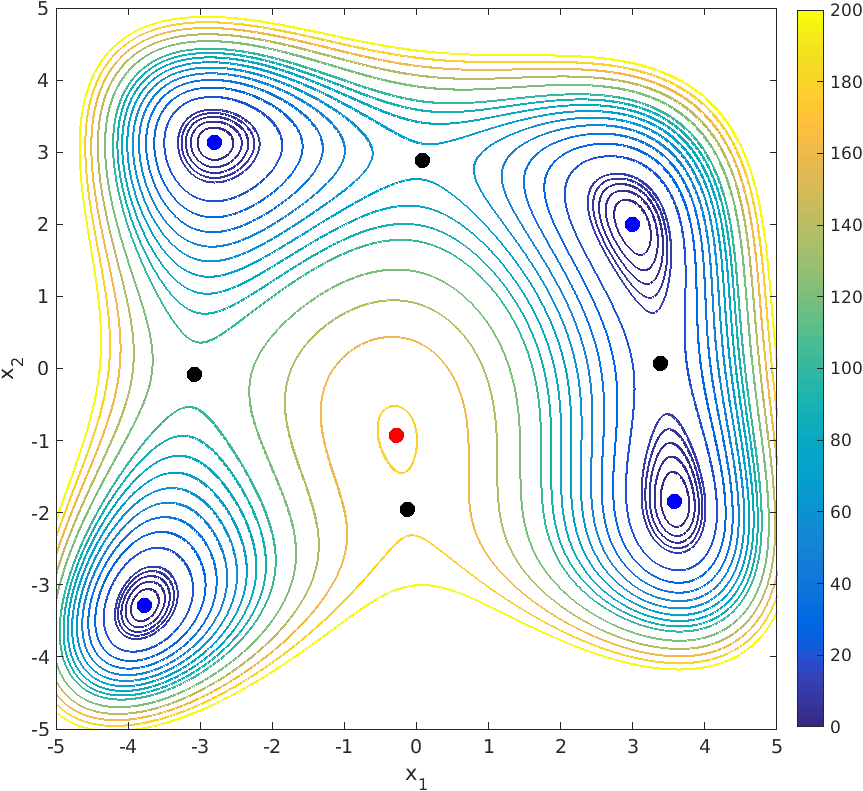
\includegraphics[width=0.8\textwidth]{../img/himmelblauContours}
\caption{Contour plot of the Himmelblau function. The blue dots are local minima, the black dots are saddle points and the red dot is a local maximum.}
\label{fig:himmelblau}
\end{figure}

\begin{table}[htb]
\centering
\begin{tabular}{l|ccc}
\hline \hline 
\# 	& $x_1$ 		& $x_2$ 			& type \\ \hline
1 	&  3			& 2				& min \\
2 	& -3.77931	& -3.28319		& min \\
3 	&  3.58443	& -1.84813		& min \\
4 	& -2.80512	& 3.13131		& min \\
5	& -0.127961	& -1.95371		& saddle \\
7	& -3.07303	& -0.0813530		& saddle \\
8	& 3.38515	& 0.0738519		& saddle \\
9	& 0.0866775	& 2.88425		& saddle \\
6	& -0.270845	& -0.923039		& max \\
\hline \hline
\end{tabular}
\caption{}
\label{tab:statPoints}
\end{table}



\subsection{Algorithms used}

Minima of the Himmelblau function will be found using four different algorithms -- steepest descent, Newton's algorithm, Quasi-Newton algorithm and Gauss-Newton algorithm -- and one trust region method -- the Levenberg-Marquardt algorithm. Having obtained the search direction the step length in each iteration will be determined using two different approaches -- Backtracking and Soft line search.

For each of the employed optimization algorithms a table will be presented with number of iterations, function evaluations and computational time (mean time in ms from 100 repetitions). For the line search methods the table will include data for both the backtracking algorithm and the soft line search. 

All code used can be found in Appendix~\ref{code:part2}.

\paragraph{Backtracking:}

This method determines the maximum step length that gives a substantial decrease along the given search direction. The algorithm, which is based in the Goldstein-Armijo condition, starts with a large step length and reduces it in each iteration while the sufficient decrease condition is not satisfied.

\begin{equation}
f(x_k + \alpha p_k) \leq f(x_k) + c_1 \alpha \nabla f_k' p_k
\label{eq:sufficientDecrease}
\end{equation}

The simplicity of this line search method is probably its main advantage. Being computationally efficient allows to use most of the machine resources to find the optimal search direction.

We wrote the algorithm and will be using it in the line search methods along with a soft line search algorithm in order to compare them and be able to point out their advantages and disadvantages.

\paragraph{Soft line search:}

Evaluating the function along the direction of search in order to find a step length that will give a sufficient decrease in the function value, before actually moving to the next iteration, has been proved to be greatly efficient in most optimization problems.

Soft line search algorithms try to find a step length that first satisfies the sufficient decrease condition (equation \ref{eq:sufficientDecrease}) and second prevents the algorithm from taking too short steps (equation \ref{eq:curvature}). While the former makes sure that we are moving towards a minimum, the latter, known as curvature condition, tries to avoid unnecessary iterations knowing that larger steps will lead us faster to the solution.


\begin{equation}
\nabla f(x_k + \alpha p_k)' p_k  \geq c_2 \nabla f_k' p_k
\label{eq:curvature}
\end{equation}

Line search algorithms start from an initial interval and reduce it in order to get to a point that matches the mentioned criteria, also known as Wolfe conditions.
 
As we said before, it is not advisable to look too close into the interval because it may waste resources that could better be used to find a more optimal search direction. Accordingly, we decided to include in our code a soft line search algorithm  that can be found in IMM Optibox.


\subsection{Steepest descent}

This algorithm is mainly based in the intuitive thinking that the fastest way to get down a slope is by choosing the direction where it decreases most rapidly, that is, the direction whose slope is minimum. 

For a continuous and differentiable function we know that this direction is given by $-\nabla f_k$, which can be shown to be orthogonal to the contours of the function. 

The direction, which changes every time depending on the place where the previous point has landed, guarantees to produce a decrease in the function. Knowing this, we can choose our step length in each iteration using a line search algorithm and find a local minimum to the function after some iterations.

We have implemented and tested our steepest descent algorithm from different starting points and using two different line search methods (backtracking and soft line search). Figure \ref{fig:steepest} shows a contour plot of Himmelblau function where the red and black lines represent the convergence sequence of the algorithm for the two line search methods from three different starting points (1,1), (1,-1) and (-1,0).

\begin{figure}[htb]
\centering
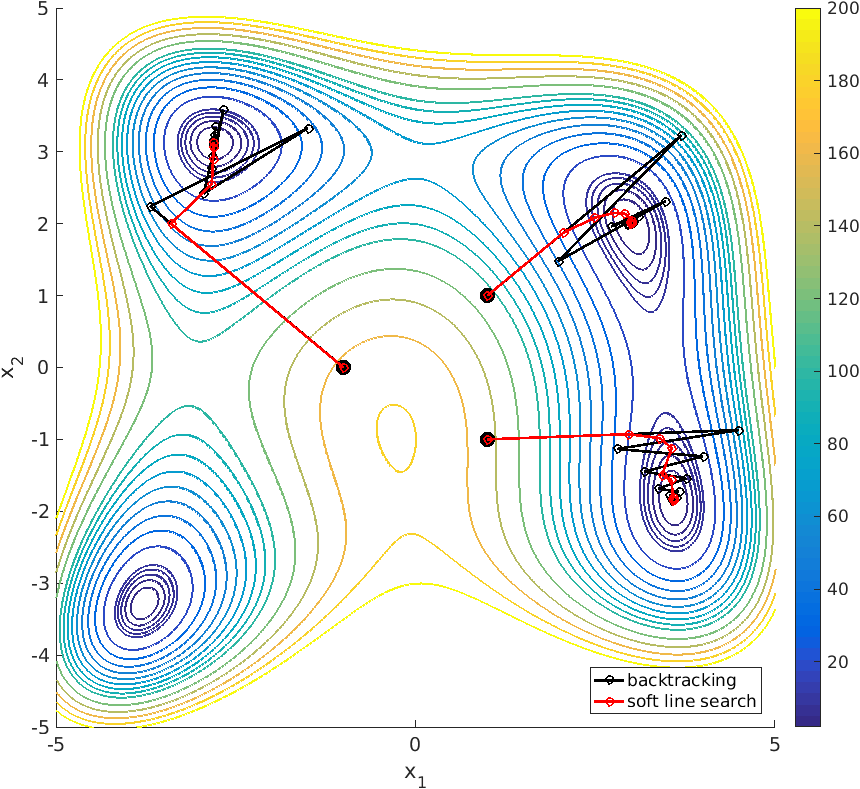
\includegraphics[width=0.7\textwidth]{../img/steepestDescent}
\caption{The steepest descent algorithm on the Himmelblau function from the starting point (1,1), (1,-1) and (-1,0).}
\label{fig:steepest}
\end{figure}

\begin{figure}[htb]
\centering
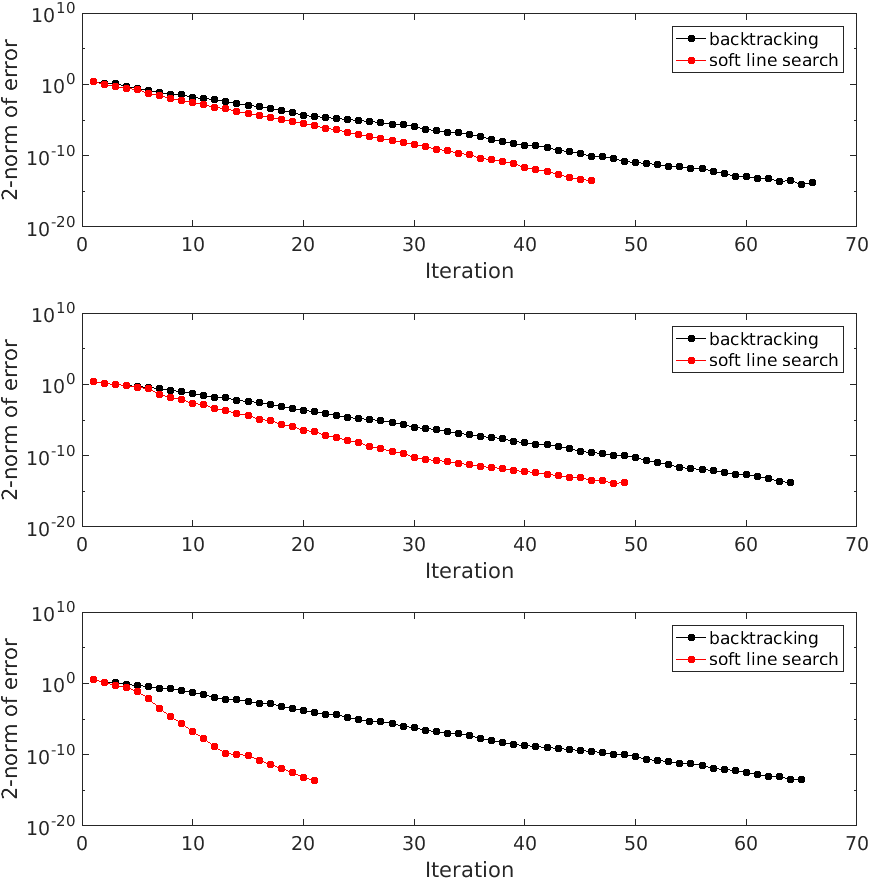
\includegraphics[width=0.7\textwidth]{../img/steepestDescentError}
\caption{Error plot for the steepest descent algorithm on the Himmelblau function. Plots are from starting points (1,1), (1,-1) and (-1,0) respectively.}
\label{fig:rateConvSteepest}
\end{figure}


The number of iterations and line search evaluations are presented in table \ref{tab:steepest}. We can see from the table and also from the graph in figure \ref{fig:rateConvSteepest} that the soft line search algorithm requires fewer iterations and function evaluations to find a minimum. However, the elapsed time is close to the same for both the soft line search and the backtrack algorithm, which means that even though the number of line search evaluations is obviously smaller, soft line search is computationally more demanding than the backtracking algorithm for each step. Even though each iteration is quicker with the backtracking algorithm, the soft line search is still faster for all the examined starting points.

Figure~\ref{fig:rateConvSteepest} indicates that the steepest descent algorithm has a linear rate of convergence for both backtracking and soft line search, which is consistent with the provided material.

\begin{table}[htb]
\centering
\begin{tabular}{l|ccc|ccc|ccc} \hline \hline 
& \multicolumn{3}{c}{$x_0 = (1,1)$} & \multicolumn{3}{c}{$x_0 = (1,-1)$} & \multicolumn{3}{c}{$x_0 = (-1,0)$} \\ 
Method & Iter & Evals & Time & Iter & Evals & Time & Iter & Evals & Time \\ \hline 
Backtracking & 66 & 3326 & 24.0 & 64 & 3028 & 19.2 & 65 & 3145 & 20.4 \\ 
Soft line search & 46 & 182 & 17.1 & 49 & 232 & 16.9 & 21 & 92 & 7.4 \\ 
\hline \hline 
\end{tabular} 

\caption{Summary of the steepest descent algorithm on the Himmelblau function}
\label{tab:steepest}
\end{table}


\subsection{Newton's algorithm}

The method derives from Taylor's quadratic approximation of a function in some neighborhood of a given point.

\begin{equation}
f (x_k + p) \approx f_k + p' \nabla f_k + \frac{1}{2}
p' \nabla^2 f_k p
\label{eq:taylor}
\end{equation}


If we assume that $\nabla^2 f_k$ is positive definite, Newton direction can be found by minimizing the equation above. The minimizer of the approximation is nothing but the next point in the iteration and therefore we can write newton direction as:

\begin{equation}
p_k = -(\nabla^2 f_k)^{-1} \nabla f_k
\label{eq:newtondir}
\end{equation}


If the Hessian ($\nabla^2 f$) stays always positive definite Newton direction can be used in order to find a local minimizer of the function. The method will be particularly favourable when the function and its quadratic approximation are close to each other.
The problem arises when the Hessian matrix is not positive definite, in those cases the direction can be no longer thought to satisfy the descent condition.

Computing the Hessian is known to be computationally demanding and although Newton’s method presents usually quadratic rate of convergence this could cause a great problem whenever the resources are poor or limited.

We have implemented the algorithm for Himmelblau function, and again we have used the two line search methods to find the optimal step length. The sequence of convergence for the two methods is represented in figure~\ref{fig:newton} where the starting points\footnote{Different starting points where chosen for Newton's algorithm compared to the other ones used, since the soft line search did not converge for any of the ones previously chosen.} are (-2,0), (1,-1) and (-4,-2). In this particular case we see that the method does not even converge when using soft line search and starting from (1,-1). A major problem of Newton method is its poor rate of global convergence. In this example, Newton direction is pointing towards a positive slope and therefore soft line search algorithm is unable to find a point that satisfies the sufficient decrease condition.

\begin{figure}[htb]
\centering
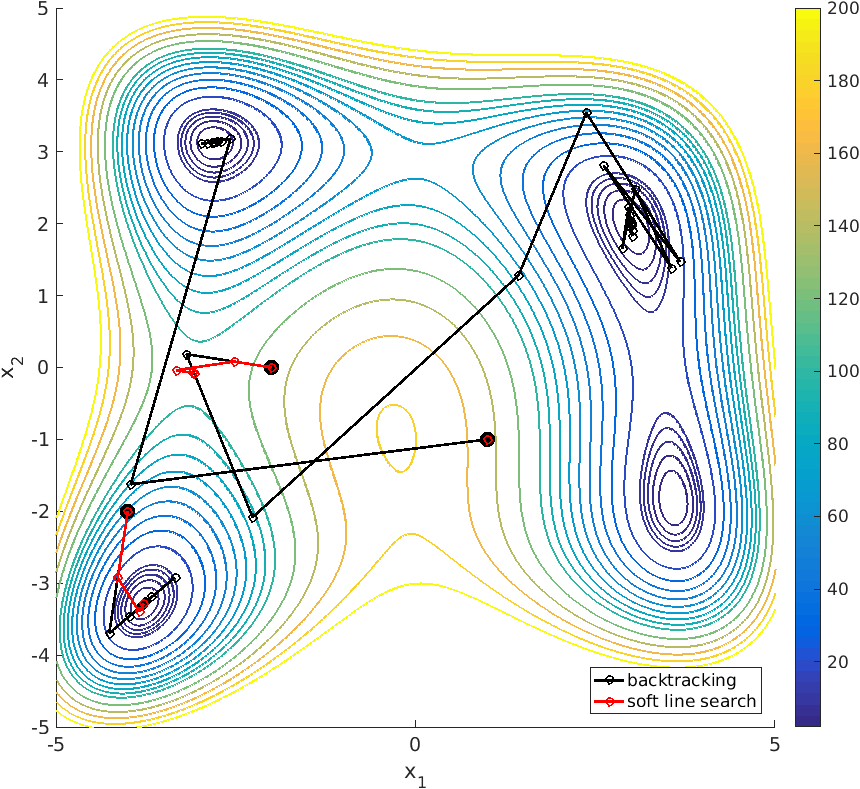
\includegraphics[width=0.7\textwidth]{../img/newton}
\caption{Newton's algorithm on the Himmelblau function from the starting point (-2,0), (1,-1) and (-4,-2).}
\label{fig:newton}
\end{figure}

\begin{figure}[htb]
\centering
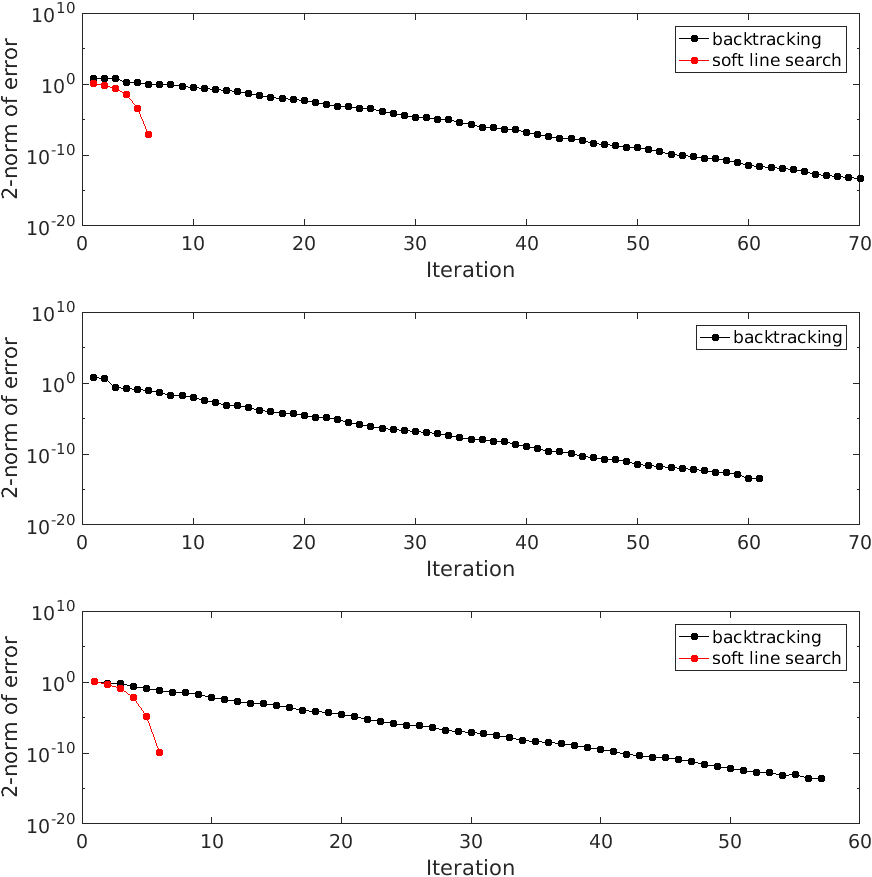
\includegraphics[width=0.7\textwidth]{../img/NewtonError}
\caption{Error plot for Newton's algorithm on the Himmelblau function. Plots are from starting points (-2,0), (1,-1) and (-4,-2) respectively.}
\label{fig:rateConvNewton}
\end{figure}

Using backtracking algorithm we set the initial step length to five in order to see if we could overcome the positive slope. In figure~\ref{fig:newton} it is seen that the backtracking algorithm converges for all of the starting points, but for (1,-1) and (-2,0) it converges to a stationary point which is far from the starting point. 

When starting from (-2,0) the soft line search sequence ends up finding a saddle point. Converging towards a maximizer or a saddle point is known to be another disadvantage of Newton method.
 
Table \ref{tab:newton} summarizes the performance for the three different starting points. Now the timing values are much shorter when the algorithm finds a solution using soft line search. This means that the use of backtracking can be only justified whenever the initial step length needs to be very large to make the algorithm converge.

\begin{table}[H]
\centering
\begin{tabular}{l|ccc|ccc|ccc} \hline \hline 
& \multicolumn{3}{c}{$x_0 = (-2,0)$} & \multicolumn{3}{c}{$x_0 = (1,-1)$} & \multicolumn{3}{c}{$x_0 = (-4,-2)$} \\ 
Method & Iter & Evals & Time & Iter & Evals & Time & Iter & Evals & Time \\ \hline 
Backtracking & 70 & 3054 & 22.0 & 61 & 3051 & 21.3 & 57 & 2822 & 22.7 \\ 
Soft line search & 6 & 7 & 2.0 & 10000 & 0 & 2455.1 & 6 & 8 & 2.2 \\ 
\hline \hline 
\end{tabular} 

\caption{Summary of Newton's algorithm on the Himmelblau function}
\label{tab:newton}
\end{table}

The convergence rate is illustrated in figure \ref{fig:rateConvNewton}. Newton's method present clear quadratic rate of convergence when using the soft line search for the two starting points where it does converge -- (-2,0) and (-4,-2). For the backtracking algorithm the convergence rate seems linear. 

\subsection{Quasi-Newton algorithm}

We have already pointed out that one of the main inconveniences of Newton's method is the large employ of computer resources, mainly derived from computing the Hessian. Quasi-Newton algorithms appeared in order to optimize such demanding computations. These methods try to give an approximation using the gradient in each iteration which is often much faster to calculate. This alternative usually requires less CPU-time while keeping a similar rate of convergence. 

In the first iteration the Hessian is substituted by the identity matrix which makes the search direction become the gradient or steepest descent direction. This is not an issue, since the steepest descent normally shows a great rate of global convergence for points which are far from minimums.

The approximations gather from the fact that changes in the gradient ($\nabla f$) give information about the Hessian along the search direction. From Taylor's approximation of a region where the Hessian is positive definite, it can be shown that:

\begin{equation}
\nabla^2 f_{k+1} (x_{k+1} - x_k) \approx \nabla f_{k+1} - \nabla f_k
\label{eq:secantCon1}
\end{equation}

Equation (\ref{eq:secantCon1}) is known as the secant condition and can also be written as:

\begin{equation}
B_{k+1} s_k = y_k
\label{eq:secantCon2}
\end{equation}

Where:


\begin{gather}
s_k = x_{k+1}-x_k \\
y_k = \nabla f_{k+1} - \nabla f_k
\label{eq:secantCon3}
\end{gather}

This, along with the conditions that $B$ has to preserve the hessian symmetry and that the difference between two successive approximations ($B_k - B_{k+1}$) must have low rank, allowed to formulate different approximations to the Hessian matrix.
In our algorithm we used the BFGS updating formula:

\begin{equation}
B_{k+1} = B_k - \frac{B_k s_k s_k' B_k}{s_k' B_k s_k} + \frac{y_k y_k'}{y_k' s_k}
\label{eq:BFGS}
\end{equation}

Figure \ref{fig:quasiNewton} illustrates the set of steps that the algorithm takes before finding a minimum from (1,1), (1,-1) and (-1,0). The plot shows that Newton's method lack of convergence has now disappeared and the iteration process is able to determine a local minimum from all the examined starting points.

\begin{figure}[htb]
\centering
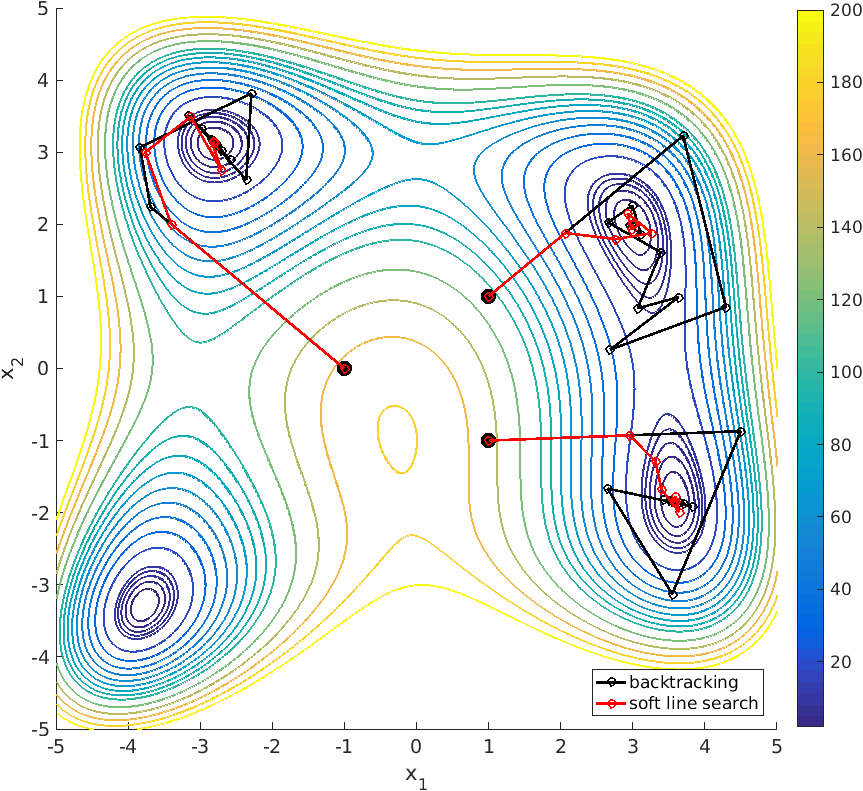
\includegraphics[width=0.7\textwidth]{../img/quasiNewton}
\caption{Quasi Newton algorithm on the Himmelblau function from the starting point (1,1), (1,-1) and (-1,0).}
\label{fig:quasiNewton}
\end{figure}

\begin{figure}[htb]
\centering
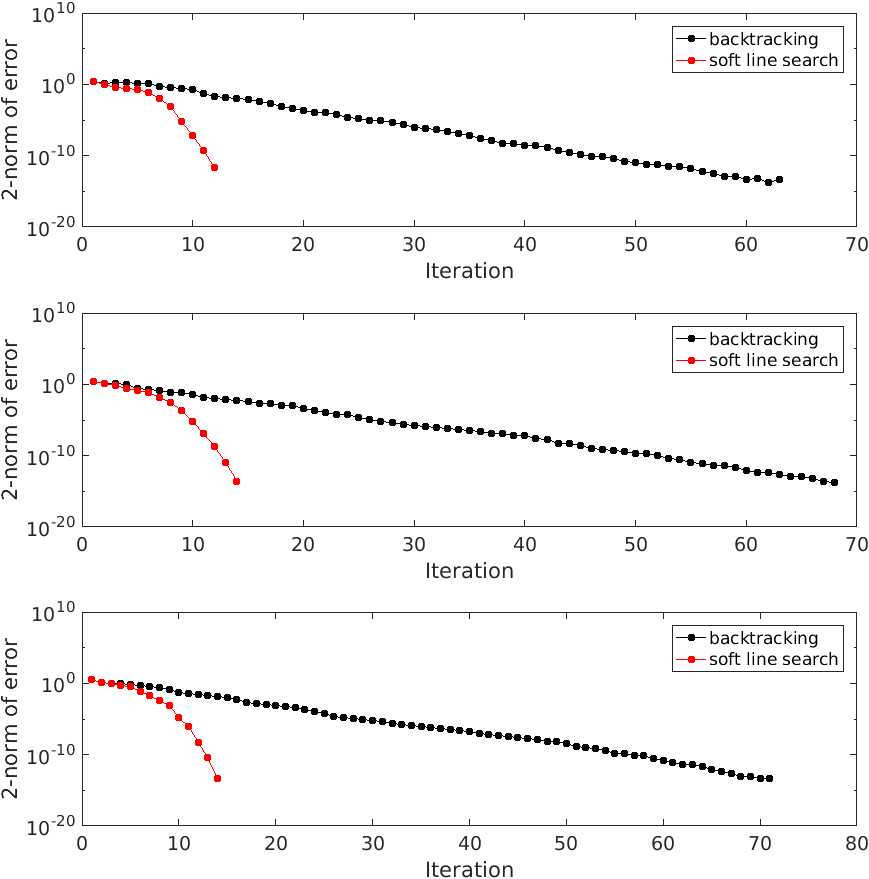
\includegraphics[width=0.7\textwidth]{../img/quasiNewtonError}
\caption{Error plot for Quasi Newton algorithm on the Himmelblau function. Plots are from starting points (1,1), (1,-1) and (-1,0) respectively.}
\label{fig:rateConvQuasiNewton}
\end{figure}

From figure~\ref{fig:rateConvQuasiNewton} we can conclude that, despite the fact that the algorithm is not computing the exact Hessian but an approximation, the rate of convergence appears to be almost quadratic (at least for the soft line search) while the algorithm has the ability to converge from a wider range of starting points. The timing values in table~\ref{tab:quasiNewton} seem to be larger than for Newton algorithm, this is due to the fact that in our code we are just evaluating the Hessian and not computing it in every iteration. However, having an expression for the Hessian matrix may not be a possibility in some problems, where it would have to be calculated every time.

\begin{table}[H]
\centering
\begin{tabular}{l|ccc|ccc|ccc} \hline \hline 
& \multicolumn{3}{c}{$x_0 = (1,1)$} & \multicolumn{3}{c}{$x_0 = (1,-1)$} & \multicolumn{3}{c}{$x_0 = (-1,0)$} \\ 
Method & Iter & Evals & Time & Iter & Evals & Time & Iter & Evals & Time \\ \hline 
Backtracking & 63 & 2971 & 23.1 & 68 & 3221 & 22.3 & 71 & 3205 & 26.6 \\ 
Soft line search & 12 & 17 & 4.4 & 14 & 21 & 4.2 & 14 & 18 & 4.9 \\ 
\hline \hline 
\end{tabular} 

\caption{Summary of the Quasi Newton algorithm on the Himmelblau function}
\label{tab:quasiNewton}
\end{table}

\subsection{Gauss-Newton algorithm}

\begin{figure}[htb]
\centering
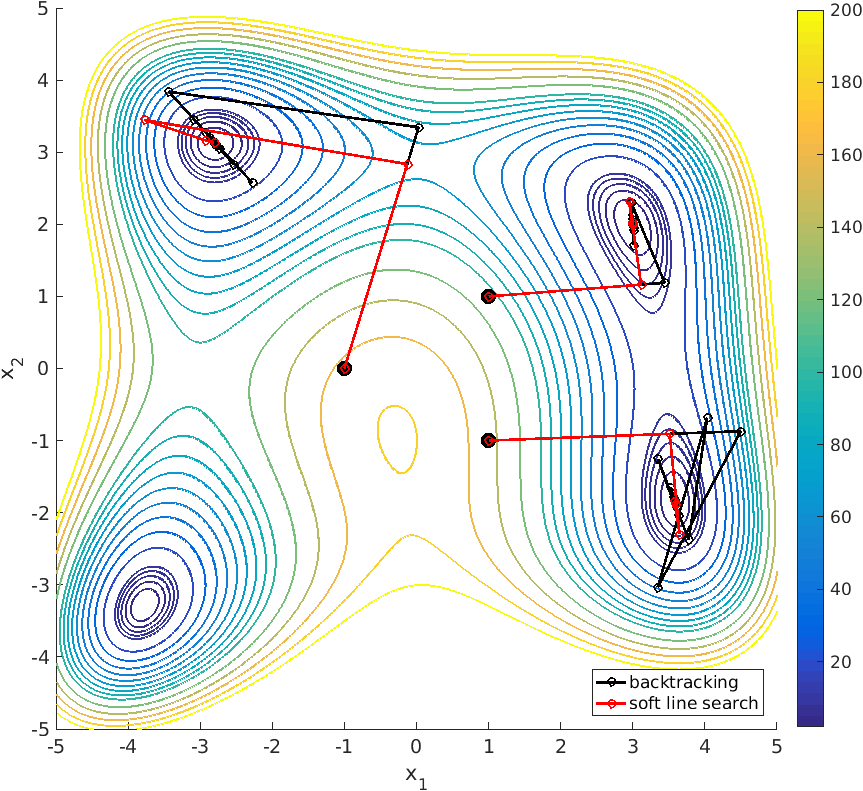
\includegraphics[width=0.7\textwidth]{../img/gaussNewton}
\caption{Gauss-Newton algorithm on the Himmelblau function from the starting point (1,1), (1,-1) and (-1,0).}
\label{fig:gaussNewton}
\end{figure}

\begin{figure}[htb]
\centering
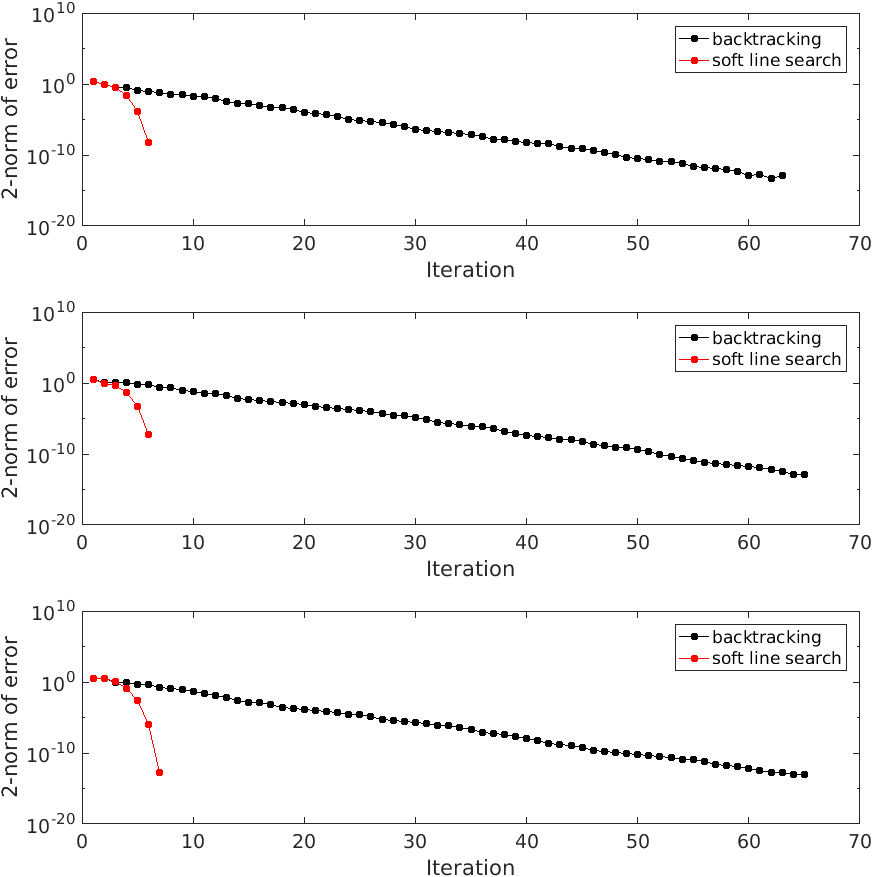
\includegraphics[width=0.7\textwidth]{../img/gaussNewtonError}
\caption{Error plot for Gauss-Newton algorithm on the Himmelblau function. Plots are from starting points (1,1), (1,-1) and (-1,0) respectively.}
\label{fig:rateConvGaussNewton}
\end{figure}

One important application of the least squares problem is the solution of a nonlinear systems of equations. We need to reformulate our optimization problem so it takes the form of: 

\begin{equation}
\text{min} \left\Vert r(x) \right\Vert_2^2
\label{eq:leastSq}
\end{equation}

By visual inspection of Himmelblau function, we see that equation \ref{eq:himm} can be written as: 

\begin{equation}
f(x) = \left\Vert r(x) \right\Vert_2^2 \\
\Rightarrow
r(x) = r(x_1,x_2) = \begin{pmatrix}
x_1^2 + x_2 - 11 \\ x_1 + x_2^2 - 7
\end{pmatrix} 
\label{eq:gaussNewton1}
\end{equation}

It can be easily shown that the gradient can be expressed in terms of the Jacobian matrix as:

\begin{equation}
\nabla f(x) = J(x)' r(x)
\label{eq:gaussNewton2}
\end{equation}

Deriving the above expression the Hessian takes the form of:

\begin{equation}
\nabla^2 f(x) = J(x)' J(x) + \sum_{i=1}^{m} r_i(x) \nabla^2 r_i(x)
\label{eq:gaussNewton3}
\end{equation}

Gauss-Newton algorithm can be viewed as a modification of Newton direction, where the Hessian is approximated by neglecting the second term in equation \ref{eq:gaussNewton3}. This approximation will be valid whenever the problem is only mildly nonlinear or the residuals at the solution are small.

\begin{equation}
\left(J(x_k)' J(x_k)\right)  p_k = - J(x_k)' r(x_k) \\
\Rightarrow p_k = - J(x_k)^{-1} r(x_k)
\label{eq:gaussNewton4}
\end{equation}


where $J(x_k)$ is the Jacobian evaluated in $x_k$

\begin{equation}
J(x) = \begin{pmatrix}
\frac{dr}{dx_1} \frac{dr}{dx_2}
\end{pmatrix}
= \begin{pmatrix}
2 x_1 & 1 \\
1 & 2 x_2
\end{pmatrix}
\end{equation}

The method makes the algorithm much more efficient, since once we have computed the gradient we can immediately obtain the approximation to the Hessian. Moreover, as long as the first term in equation \ref{eq:gaussNewton3}, ($J(x)'J(x)$), is much larger than the second, the algorithm will preserve Newton's quadratic convergence.

Finally, if $J(x)$ has full rank and the gradient is different from 0, we can assure that the search direction is a descent direction and thus, our method will converge to a minimum.

In figure~\ref{fig:gaussNewton} the convergence sequence can be seen from the three starting points. It is seen that this variation of Newton's algorithm can converge from all the starting points -- contrary to Newton's algorithm presented using the Hessian. From figure~\ref{fig:rateConvGaussNewton} it is seen, that the quadratic convergence of Newton's algorithm is preserved (at least for the soft line search). The required number of iterations to converge along with the computational time (table~\ref{tab:gaussNewton}) is similar to Newton's algorithm and this is because the residuals are close to 0 when near the solution. Consequently, the approximation of the Hessian happens to be acceptable, since the first term of equation \ref{eq:gaussNewton3} is significantly greater than the second term.

\begin{table}[H]
\centering
\begin{tabular}{l|ccc|ccc|ccc} \hline \hline 
& \multicolumn{3}{c}{$x_0 = (1,1)$} & \multicolumn{3}{c}{$x_0 = (1,-1)$} & \multicolumn{3}{c}{$x_0 = (-1,0)$} \\ 
Method & Iter & Evals & Time & Iter & Evals & Time & Iter & Evals & Time \\ \hline 
Backtracking & 63 & 2983 & 20.1 & 65 & 2819 & 19.2 & 65 & 3046 & 19.8 \\ 
Soft line search & 6 & 10 & 1.9 & 6 & 11 & 1.9 & 7 & 12 & 2.0 \\ 
\hline \hline 
\end{tabular} 

\caption{Summary of the Gauss-Newton algorithm on the Himmelblau function}
\label{tab:gaussNewton}
\end{table}

\subsection{Levenberg-Marquardt}

\begin{figure}[htb]
\centering
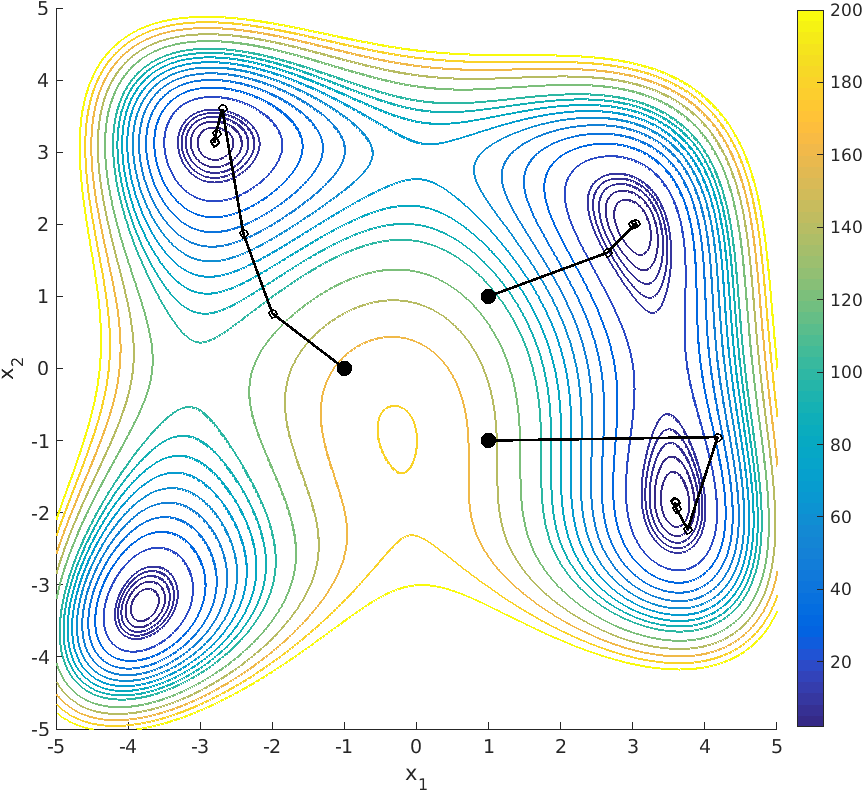
\includegraphics[width=0.7\textwidth]{../img/LM}
\caption{Levenberg-Marquardt algorithm on the Himmelblau function from the starting point (1,1), (1,-1) and (-1,0).}
\label{fig:LM}
\end{figure}

\begin{figure}[htb]
\centering
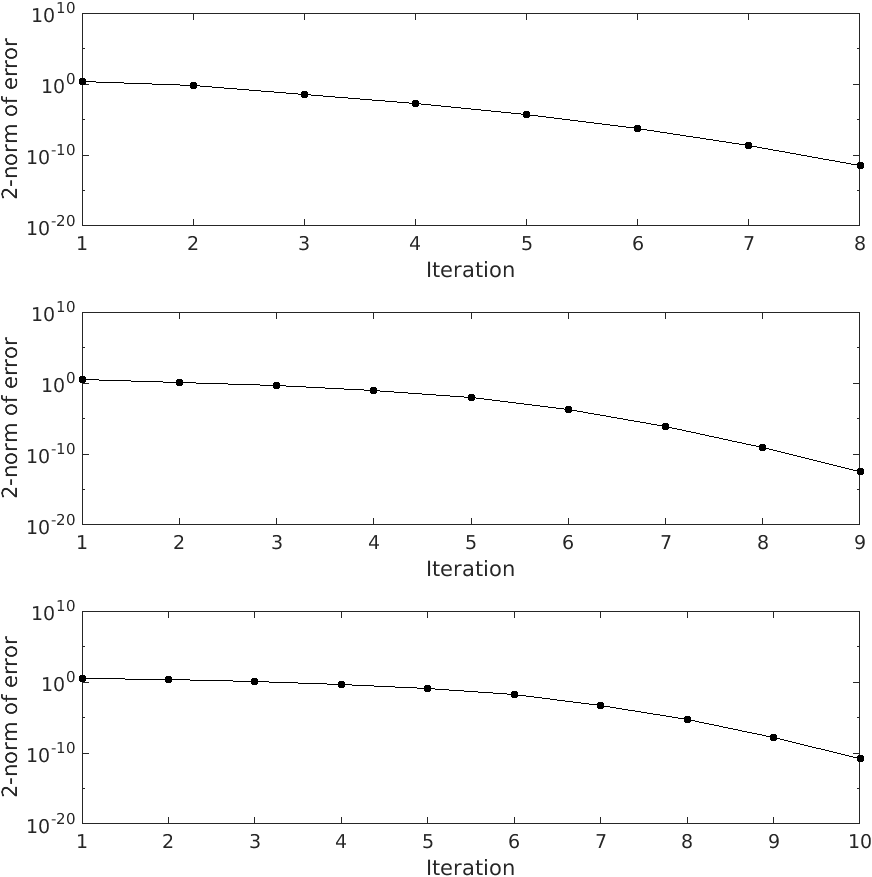
\includegraphics[width=0.7\textwidth]{../img/LMError}
\caption{Error plot for Levenberg-Marquardt algorithm on the Himmelblau function. Plots are from starting points (1,1), (1,-1) and (-1,0) respectively.}
\label{fig:rateConvLM}
\end{figure}

Levenberg-Marquardt method can be treated as one of the many damped newton algorithms.

In order to face the global convergence problem of Newton's method Damped Newton algorithms try to combine the safe and global convergence properties of steepest descent direction, whenever the iteration is far from the solution, and the quadratic convergence rate of Newton's algorithm when the sequence is close to a local minimum.

This is done by modifying the Newton direction as shown in equation \ref{eq:dampedNewton}.

\begin{equation}
p_k = -(\nabla^2 f_k + \mu I)^{-1} \nabla f_k
\label{eq:dampedNewton}
\end{equation}

Where the damping parameter ($\mu$), which is always greater than 0, is updated in every iteration.

We see that when $\mu = 0$ the search direction is equal to Newton's direction and as $\mu$ gets larger equation \ref{eq:dampedNewton} looks more similar to steepest descent direction divided by $\mu$. Therefore, ideally, $\mu$ will be bigger when the algorithm iterates somewhere far from a local minimum and it will be 0 or close to 0 when being around the solution.

Damped Newton algorithms differ in the way they update $\mu$, specifically Levenberg-Marquardt method makes sure that the sequence moves towards a minimum by checking that the matrix $\nabla^2 f_k + \mu I$ is positive definite before taking the next step. The damped factor is increased when the matrix is not positive definite. 

By updating the damping parameter, Levenberg-Marquardt method tries to influence both search direction and step length, thus the use of a line search algorithm turns to be unnecessary.

Again the optimization problem can be transformed into a least squares problem and then, equation \ref{eq:dampedNewton} can be written as, where the term $J(x_k)' J(x_k)$ is an approximation to the Hessian:

\begin{equation}
p_k = -(J(x_k)' J(x_k) + \mu I)^{-1} J(x_k) r(x_k)
\label{eq:LM}
\end{equation}

In figure~\ref{fig:LM} the convergence paths can be seen from the three starting points. The Levenberg-Marquardt seems to converge quadratically for all the starting points (figure~\ref{fig:rateConvLM}). Even though it takes a similar number of iterations as some of the line search methods, it is seen (table~\ref{tab:LM}) that the computational time is much lower for the Levenberg-Marquardt algorithm. This is because the algorithm does not need any further method to determine the step length.

\begin{table}[H]
\centering
\begin{tabular}{ccc|ccc|ccc} \hline \hline 
\multicolumn{3}{c}{$x_0 = (1,1)$} & \multicolumn{3}{c}{$x_0 = (1,-1)$} & \multicolumn{3}{c}{$x_0 = (-1,0)$} \\ 
Iter & Evals & Time & Iter & Evals & Time & Iter & Evals & Time \\ \hline 
8 & 16 & 0.42 & 9 & 18 & 0.43 & 10 & 22 & 0.55 \\ 
\hline \hline 
\end{tabular} 

\caption{Summary of the Levenberg-Marquardt algorithm on the Himmelblau function}
\label{tab:LM}
\end{table}


\subsection{Comparison of algorithms}

As a conclusion for the optimization problem, we have gathered the results of all our algorithms in table \ref{tab:all} along with some outputs obtained from Matlab optimization function fminunc. 

We have mentioned that although requiring many iterations, the intuitive steepest descent method is always able to find a solution even when starting from points which are far from local minimums.  If we look at the number of iterations and function evaluations of steepest descent we realize that the values are considerably larger than for the rest of the algorithms.

\begin{table}[H]
\centering
\begin{tabular}{l|ccc|ccc|ccc} \hline \hline 
{\bf Algorithm} & \multicolumn{3}{c}{$x_0 = (1,1)$} & \multicolumn{3}{c}{$x_0 = (1,-1)$} & \multicolumn{3}{c}{$x_0 = (-1,0)$} \\ 
& Iter & Evals & Time & Iter & Evals & Time & Iter & Evals & Time \\ \hline 
Steepest Descent & 46 & 182 & 17.1 & 49 & 232 & 16.9 & 21 & 92 & 7.4 \\
\hline
Quasi Newton & 12 & 17 & 4.4 & 14 & 21 & 4.2 & 14 & 18 & 4.9 \\ 
\hline
Gauss-Newton & 6 & 10 & 1.9 & 6 & 11 & 1.9 & 7 & 12 & 2.0 \\ 
\hline
Levenberg-Marquardt & 8 & 16 & 0.42 & 9 & 18 & 0.43 & 10 & 22 & 0.55 \\
\hline
fminunc & 7 & 8 & 17.3 & 8 & 9 & 17.7 & 7 & 8 & 16.6 \\ 
\hline \hline
& \multicolumn{3}{c}{$x_0 = (-2,0)$} & \multicolumn{3}{c}{$x_0 = (1,-1)$} & \multicolumn{3}{c}{$x_0 = (-4,-2)$} \\ 
& Iter & Evals & Time & Iter & Evals & Time & Iter & Evals & Time \\ \hline 
Newton & 6 & 7 & 2.0 & 10000 & 0 & 2455.1 & 6 & 8 & 2.2 \\ 
\hline \hline
\end{tabular} 

\caption{Summary of the methods discussed. For the line search methods -- Steepest descent, Quasi Newton, Gauss-Newton and Newton -- only the results from the soft line search are included. The results from fminunc (using Levenberg-Marquardt) from matlab are also included. Notice that all algorithms have the same starting points except Newton's algorithm, since it failed to converge for all of them. }
\label{tab:all}
\end{table}

On the other hand, we showed that apart from being computationally demanding Newton method presents a lack of global convergence, a good example of this is the starting point (-1,1) where Newton algorithm is unable to find a solution. However, when iterating around a minimum (starting point -4,-2) the convergence turns out to be quadratic and the number of iterations is low. We said that the iterations could sometimes lead the sequence to a maximum or a saddle point, as it occurs when starting from (-2,0). 

Quasi Newton algorithm appeared as an efficient alternative to Newton method, where the Hessian is approximated in every iteration. Obviously, that comes along with a lower convergence rate which can be seen if we compare the number of iterations and function evaluations for both algorithms. Yet, the values are lower than for steepest descent while it potentially employs less resources than Newton method, as it does not compute the Hessian. 

Again, we would like to remark that in our algorithms we are using an expression for evaluating the Hessian, which avoids tedious computations. Therefore, the improvement of using Quasi-Newton approximation instead of the exact Hessian matrix cannot be seen by looking at the timing values.

Treating the optimization problem as a least square problem allowed us to write an algorithm that gives an approximation to the Hessian by using the Jacobian matrix. Gauss-Newton algorithm is particularly advisable when the residuals are close to 0, which occurs when the sequence is near a minimum. It also offers good computation results because there is no need to calculate second derivatives. The low number of iterations and function evaluations for any of the starting points presented in table \ref{tab:all} prove that the algorithm is totally suitable for our minimization problem.

Levenberg-Marquardt combines steepest descent's global convergence properties with Newton's quadratic convergence by adding the damping factor to the Hessian matrix. The factor can be used to control both direction and step length and thus we did not use a line search method in this algorithm. The values show that while keeping the number of iterations and function evaluations low, the algorithm is much faster than the rest as it does not need an inner loop to find the step length in every iteration.

Finally, from the results obtained by running fminunc function (which was set to use a Levenberg-Marquardt method), it can be seen that, although the number of iterations and evaluations can be reduced compared to our implementation, the computational time is much higher.